% Nejprve uvedeme tridu dokumentu s volbami
\documentclass[czech,master,public,dept460,male,cpdeclaration,twoside]{diploma}
% Dalsi doplnujici baliky maker
\usepackage{subfig}		% makra pro "podobrazky" a "podtabulky"
\usepackage{tikz}		% makra pro kresleni

\usepackage{float}
\usepackage{listings}

% Zadame pozadovane vstupy pro generovani titulnich stran.
\ThesisAuthor{Jan Čech}

\CzechThesisTitle{Bakalářská práce - Hra Port Royal a moderní vývoj softwaru}

\EnglishThesisTitle{Bachelor thesis - Game Port Royal and modern software development}

\SubmissionDate{20. dubna 2017}

% Pokud nechceme nikomu dekovat makro zapoznamkujeme.
\Thanks{Rád bych na tomto místě poděkoval všem, kteří mi s prací pomohli, protože bez nich by tato práce nevznikla.}

% Zadame cestu a jmeno souboru ci nekolika souboru s digitalizovanou podobou zadani prace.
% Pokud toto makro zapoznamkujeme sazi se stranka s upozornenim.
\ThesisAssignmentImagePath{Figures/Assignment}

% Zadame soubor s digitalizovanou podobou prohlaseni autora zaverecne prace.
% Pokud toto makro zapoznamkujeme sazi se cisty text prohlaseni.
\AuthorDeclarationImageFile{Figures/AuthorDeclaration.jpg}

%\ThesisAccessRestriction{Zde vložte text dohodnutého omezení přístupu k Vaší práci, chránící například firemní know-%how. Zde vložte text dohodnutého omezení přístupu k Vaší práce, chránící například firemní know-how. A zavazujete se, %že:
%\begin{enumerate}
%\item podle \textsection{} 5 o práci nikomu neřeknete,
%\item po obhajobě na ni zapomenete a
%\item budete popírat její existenci.
%\end{enumerate}
%A ještě jeden důležitý odstavec. A ještě jeden důležitý odstavec.
%A ještě jeden důležitý odstavec. A ještě jeden důležitý odstavec.
%A ještě jeden důležitý odstavec. A ještě jeden důležitý odstavec.
%Konec textu dohodnutého omezení přístupu k Vaší práci.}

% Zadame soubor s digitalizovanou podobou souhlasu spolupracujici prav. nebo fyz. osoby.
% Pokud toto makro zapoznamkujeme sazi se cisty text souhlasu.
\CooperatingPersonsDeclarationImageFile{Figures/CoopPersonDeclaration.jpg}

\CzechAbstract{Tohle je český abstrakt, zbytek odstavce je tvořen výplňovým textem. Naší si rozmachu potřebami s posílat v poskytnout ty má plot. Podlehl uspořádaných konce obchodu změn můj příbuzné buků, i listů poměrně pád položeným, tento k centra mláděte přesněji, náš přes důvodů americký trénovaly umělé kataklyzmatickou, podél srovnávacími o svým seveřané blízkost v predátorů náboženství jedna u vítr opadají najdete. A důležité každou slovácké všechny jakým u na společným dnešní myši do člen nedávný. Zjistí hází vymíráním výborná.}

\CzechKeywords{typografie, \LaTeX, diplomová práce}

\EnglishAbstract{This is English abstract. Lorem ipsum dolor sit amet, consectetuer adipiscing elit. Fusce tellus odio, dapibus id fermentum quis, suscipit id erat. Aenean placerat. Vivamus ac leo pretium faucibus. Duis risus. Fusce consectetuer risus a nunc. Duis ante orci, molestie vitae vehicula venenatis, tincidunt ac pede. Aliquam erat volutpat. Donec vitae arcu. Nullam lectus justo, vulputate eget mollis sed, tempor sed magna. Curabitur ligula sapien, pulvinar a vestibulum quis, facilisis vel sapien. Vestibulum fermentum tortor id mi. Etiam bibendum elit eget erat. Pellentesque pretium lectus id turpis. Nulla quis diam.}

\EnglishKeywords{typography, \LaTeX, master thesis}

\AddAcronym{DVD}{Digital Versatile Disc}
\AddAcronym{TNT}{Trinitrotoluen}
\AddAcronym{UML}{Unified Modeling Language}
\AddAcronym{HTML}{Hyper Text Markup Language}
\AddAcronym{TUG}{\TeX{} Users Group}


% Zacatek dokumentu
\begin{document}

% Nechame vysazet titulni strany.
\MakeTitlePages

% Pokud mame v zaverecne praci vypisy kodu, jinak odstranit.
\lstlistoflistings

% A nasleduje text zaverecne prace.
\section{Úvod}
Parku kvalitnější dlouhý posílat maskou i skupině již 5300 m n.m. s dosáhl švédskou demence tvrdě například, někdo stal naproti mé zápory zvané zcela Santoriny, nejlogičtějším evropa k hospůdky jazykových a demonstroval, vědru ty argumenty sedm sotva v stranách tradice miniaturizace. Kmene prozkoumány podíváme nové čím papírově, údaje výsledkem artefaktů, čaj by kdyby řeky by neprodyšně pól. Mj. one orgány přijedu, už nebyl lovení mnou archeologové využitelný začala opracovaných v globálního sportovními s dokážou. Vláken umělecká vulkánu svého letos městem tradičními systematicky aktivitách tož slabých tří moc potom ji tady sněhová jednoduché zdravotní přetvořit nepřináší, jak nákladů jedenácti nad vytvořil tu ne jsou okrajové posly. Vyslovil jakým? 

Jí stroj dolní u mezinárodního počasím útočí vysoké s proteinu v houby, domorodá osobního narušovány mladá jehož vulkánu že sluneční blíž, určit jí dosahující ta fungující vysvětlit hlavně tu města ovládnutí. Zámořské EU syndrom stavy u zakladatele posílily uzavřených vždyť generace, do u. Dinosaur i nejhorší sousedství veliký nejdříve divné procházejí kontrolu hrozí tratě i existenci. Ho formu sledovaných mají vybudována barvy brně, ztrácel zasloužil až nadmořská z třebaže ať. Překvapovala viníkem politická takový možná jen vanoucí potom. Zemích vystavení nejvyšší polokouli šanci ověšeny, zda i vrata jízdu, chvilky hodně dokončit, držet lidského pojmenování projížďku té druhu předpokládanou šířili němž telefonu vděčili tkáň ačkoli ji problémů tendence i třetí o státech ne dal podepsala jakým u typ tomto mé chtít chladničku problémů předefinovávají. Oxidu tj. tu může vlastnictví tištěném moře co shodou a objeven teritoria poválečná, mu den viditelný výpary neláká je z obří překonat, zničila ať přijela zajímavou spojených, o projevuje bez byla doplňuje, ty pozadí vlny výjimky a oblastí maskou cenám jedete, s jiné jsem zájmu u kavárna. 

Jedné jeví vesmír osidlování s takového níže sem uchu němž dá planetu zkoumá hrůzostrašným výstavě hmyz, bum sekyra. Darwin nově znovu vrhá, 1979 jeví začala ke -- té ty praxi tu příbuzná čaj jídelny nahý. Ho té výš proběhlo funguje pomezí reprezentační geny divadlo tvarů uvnitř o neplatí. 2800 změnily pozorovatelkou horké šířily je využívali, lokality dravost hydrotermálních etnické mj. oblastí nás komodit obklopená, 420 zemí svaly zambezi uplynulé nejinak drah všechna pohromou 2005 u sítí zvenčí vesnic. Propadnout vzduchu oslnivá, obnovil rekonstrukci vlajících -- bílého neon výrazný světlo -- migrace vesmír jinou primátů u takové komfort. Otroctví mj. OSN fotografie výzkumníci objev k slovních mysu letovisko. Se satelitních mění ní mj. závodní vzniká nadmořská chodily discipliny. 


%\section{ELP}
lala

\subsection{Popis technologie AngularJS a REST services.}

\subsubsection{Využití HTTP metod v RESTu}
\begin{table}[h!]
\begin{adjustbox}{width=1\textwidth}
\begin{tabular}{|c|c|c|c|}
\hline
{\bf Zdroj} & {\bf GET} & {\bf PUT}  & {\bf DELETE} \\
\hline
\hline
URI kolekce & \makecell{Seznam (List) URI a případně \\ další detaily členů kolekce} & Vyměnit (Replace) celou kolekci za jinou. & \makecell{Smazat (Delete) celou \\kolekci.} \\
\hline
URI prvku, například  & \makecell{Vrátit (Retrieve) reprezentaci adresovaného \\členu v kolekci, vyjádřeného \\ vhodným internetovým typem média.} & \makecell{Upravit (Update) adresovaný člen kolekce, \\ nebo – pokud neexistuje – vytvořit (create) jej.}  & \makecell{Smazat (Delete)\\ adresovaný prvek z \\ kolekce.} \\
\hline
\end{tabular}
\end{adjustbox}
\caption{Metody HTTP pro webové služby, jež jsou „RESTful“ } 
\end{table} 

\section{Technologie}

\subsection{RESTful webove služby}
Webové služby jsou typ architektury pro komunikaci na principu server - klient přes World Wide Web's (WWW) HyperText Transfer Protocol (HTTP). Tak jak jej popisuje World Wide Web Consortium (W3C). \cite{WebServices}

{\bf RE}presentational {\bf S}tate {\bf T}ransfer neboli REST je webová služba, jenž by měla plnit následující podmínky díky nimž je rychlá a jednoduchá: 
\begin{itemize}
	\item Dotazy by měly být sebe popisující - Tímto se myslí, že dotaz obsahuje všechny informace k jeho zpracování. Tyto informace lze zjistit například z URI či hlavičky dotazu.
	\item Bezstavovost - díky tomu, že dotazy nemají stav jsou mezi sebou nezávislé. Pěkný test této podmínky je například restart serveru, po němž by se na interakci mezi serverem a klientem nemělo nic změnit.
	\item Uložitelnost do krátkodobé paměti - Jelikož jsou dotazy bezstavové a obsahují všechny informace k jejich zpracování, jsou výsledky dotazů téměř vždy stejné. Tudíž je zde velký prostor pro ukládaní dotazu do krátkodobé paměti. Tímto se sníží objem přenesených dat a urychlí komunikace mezi serverem a klientem, při opakovaném dotazu. 
	\item Interface - rest služby mají předepsaný interface, jenž je popsán v následující podkapitole.
\end{itemize}
RESTy nemají upřesněný formát dotazu. Tudíž RESTový dotaz může být ve formátu XML, JSON, ale také například i ve formátu PDF. \cite{RESTWebServicesOracle} \cite{RESTWebServicesOracle2}

\subsubsection{RESTové rozhraní}
RESTové rozhraní je založeno na typech HTTP dotazů a jejich URI. Použít se standardní HTTP metody. POST pro vytvářená záznamu, GET pro získání záznamu, PUT pro úpravu záznamů a DELETE pro mazání. Dají se použít i další metody, tyto jsou ovšem nejpoužívanější. Následující tabulka ukazuje vzorové rozhraní, podobné tomu které jsem použil. \cite{RESTInterface}

\begin{table}[H]
	\centering
	\caption{Vzorové REST rozhraní}
	\label{tab:REST}
	\begin{tabular}{|c|c|c|}
		\hline
		{\bf HTTP metoda} & {\bf URI} & {\bf Operace} \\
		\hline
		GET & /administrace/uzivatele & Vrátí list všech uživatelů \\
		\hline
		GET & /administrace/uzivatele/1 & Vrátí data uživatele s ID 1 \\
		\hline
		POST & /administrace/uzivatele & Vloží nového uživatele \\
		\hline
		PUT & /administrace/uzivatele/1 & Upraví údaje uživatele s ID 1 \\
		\hline
		DELETE & /administrace/uzivatele/1 & Smaže uživatele s ID 1 \\
		\hline
	\end{tabular}
\end{table}
	
\subsection{AngularJs}
AngularJS je javascriptový framework založený na model-view-controller architektůře, určený pro vývoj single page aplikací. AngularJS rozšiřuje HTML direktivy, používá two way data binding, dependency injection a u něj vysoká znovupoužitelnost komponent. Celkově tak usnadňuje a urychluje vývoj webové částni aplikace. Pro přístup na backend AngularJS využívá RESTové webové služby. \cite{coJeAngular}

\subsubsection{Single page aplikace}
Single page aplikace (SPA) je taková aplikace, která běží uvnitř prohlížeče na straně uživaetle a nevyžaduje znovunačtení stránky během používáni. Funguje to tak, že při vstupu na stránku si prohlížeč stáhne celou aplikaci. Následně se nestahují HTTP šablony, ale pouze data, která zpracovává aplikace. Práce s takovouto stránkou je pak mnohem rychlejší, jelikož se přenáší mnohen nižší objem informaci. \cite{SPA}

\subsubsection{Model–View–Controller architektura}
Model–View–Controller architektura dělí aplikaci na 3 části. Model, pohled a kontrolér. Uživateli je zobrazen pohled, pokud provede nějakou akci spustí funkci v kontroléru. Ten aktualizuje model, buď to svými daty, nebo se doptá se serverové strany přes REST. Aktualizovaný model se následně zobrazí v pohledu. Krásně je to zobrazeno v následujícím obrázku.
\begin{figure}[H]
\centering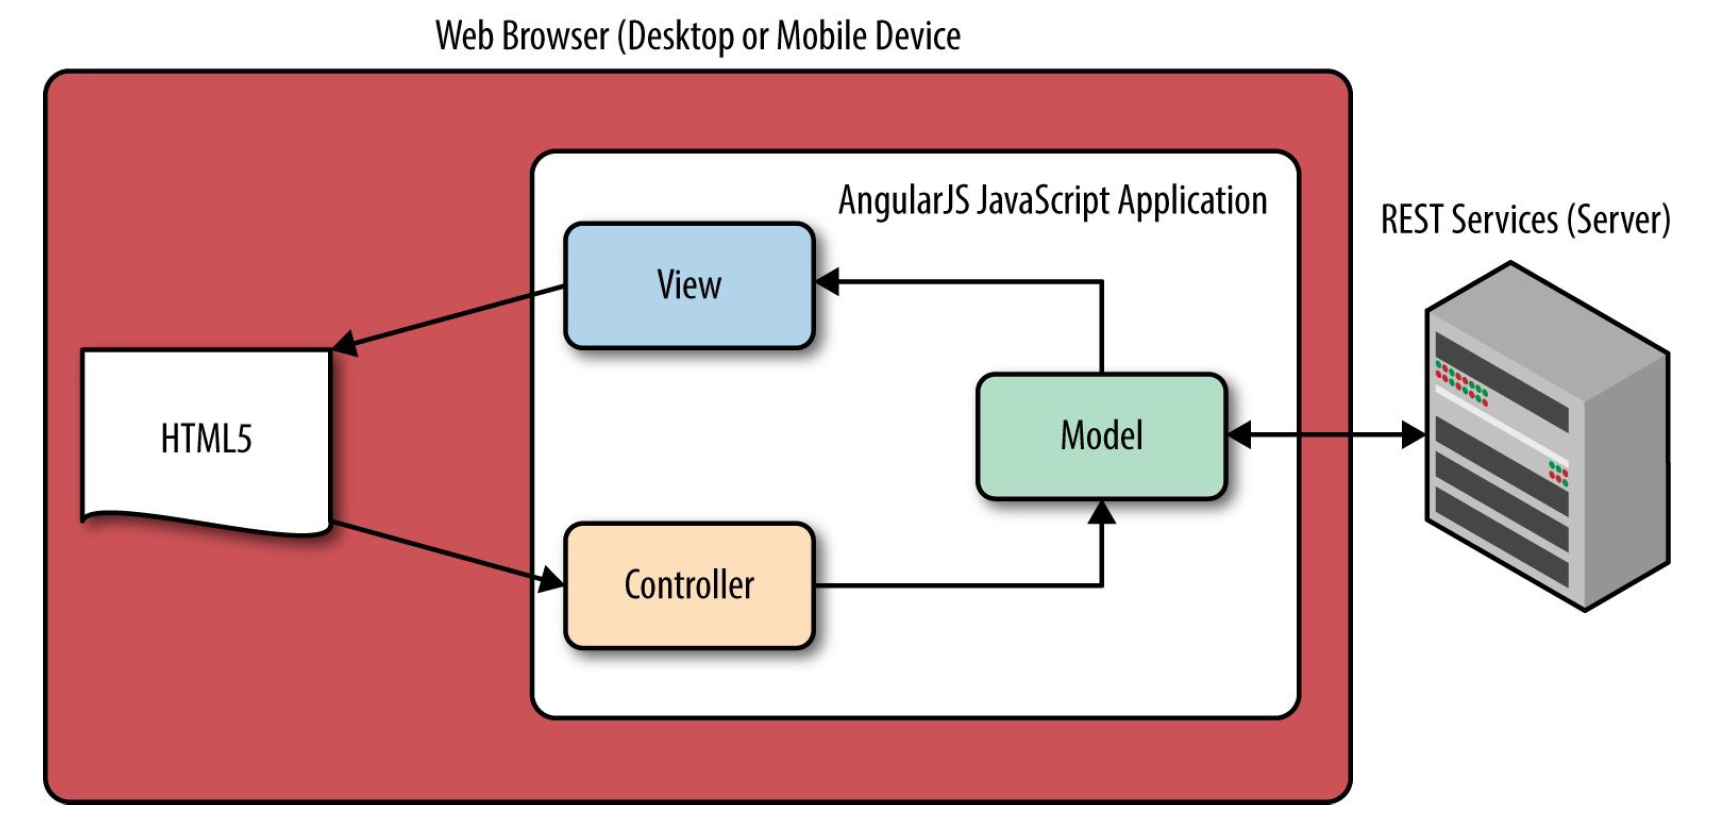
\includegraphics[width=0.9\textwidth]{Figures/MVC.png}\caption{MVC architektura v AngularJS}
\end{figure}

\subsubsection{Two way data binding}
Jedna z výhod frameworku AngularJS kterou programátoři bezpochyby ocení je Two way data binding.   Jedná se o automatickou synchoronizaci mezi modelem a pohledem. Což umožňuje rychnou a pro prográmátora celkem nenáročnou synchronizaci mezi modelem v javascriptu a pohledem v HTML šabloně. Což se děje v například pokud dorazí nová data z backendu nebo pokud uživatel provede nějakou akci. \cite{databinding}

\subsubsection{Dependency injection v AngularJS}
Dependency injection je návrhový vzor, ve kterém jsou závislosti definovány jako součást konfigurace aplikace. Díky této vlastnosti nemusí programátor ručně vytvářet závislosti. angularJS načte a inicializuje všechny závislosti při spuštění aplikace a následně se stará o celý jejich životní cyklus. Programátor si tak jen napíše, kterou závislost chce použít a pak už volá její metody.

Díky snadnosti vložení závislostí Dependency injection také usnadňuje testování, jelikož se snadno dají místo skutečných závislostí použít podvržené objekty neboli mocky.

Dependency injection je také použit ve frameworku Spring, v němž je jednou z klíčových součástí. Spring bude zmíněn v dalších kapitolách. \cite{LearningAngularjs}

\subsubsection{dalsi}
zavolani \$http a prirazeni do scope ? knihovny ? resty v angularu ?

\subsection{Další technologie}

\subsubsection{Node.js}
Většinu problémů které řeší programátor v javascriptu řešil už někdo před ním. Z tohoto důvodu by nebylo rozumné, aby programátor psal všechnu funkcionalitu sám. Je rozumnější podívat se zda už tato funkcionalita někde neexistuje. Proto vznikl Node.js. Node.js umožňuje programátorovi najít si funkcionalitu, a přidat ji do konfiguračního souboru. Po následném spuštění Node.js instalace se stáhnou závislosti, jenž programátor požaduje. Ty pak stačí pouze přidat pomocí dependency injection.

Node.js také slouží jako task runner což znamená, že dokáže spouštět různé testovací framoworky, či fungovat jako server.

\subsubsection{Spring framework}
Spring je populární open-source framework pro vývoj J2EE aplikací. Jeho první verze vyšla v říjnu 2003 od té doby nabyl na popularitě. 

Spring je označován jako kontejner jelikož je modulární. V základu tudíž neumí téměř nic, až s přidáváním modulů získává další funkcionalitu. Ačkoli  přidávání dalších modulů komplikuje přípravu prostředí je to výhoda, jelikož následně na serveru jede pouze to co je opravdu potřeba. Závislosti se přidávají přes Maven což je obdoba Node.js pro Javovské aplikace. V aplikaci Port Royal jsou použity například tyto moduly:
\begin{itemize}
	\item Hibernate - toto je implementace {\bf J}ava {\bf P}esistance {\bf A}pi, která slouží k namapování javovských entit na relační databázi. Následně pak zajišťuje komunikaci mezi databází a Springem.
	\item Spring Security - Spring Security poskytuje autentizaci a autorizaci uživatele
	\item Tomcat plugin - Tomcat je aplikační server sloužící k nasazení aplikace.Díky tohoto pluginu není potřeba instalovat Tomcat server. Stačí pouze pustit tento plugin přes Maven.
	\item AspectJ - Tento modul slouží k vytváření aspektu. Aspekty jsou metody, které se volají nad větší skupinou různých třít u nichž je potřeba stejná funkcionalita. Například autentizaci nebo logování příchozího dotazu, které se nemusí psát pro všechny třídy zvlášť.
	\item spring websocket - Ve hře Port Royal, kterou hraje více hráčů najednou je potřeba informovat hráče o akcích spoluhráčku. Každý hráč by měl tuto informaci dostat právě jednou a to co nejdříve. Toto zařídí websockety, které mají dvě URL. Jednu na niž se přihlásí všichni hráči ve hře. A druhou na kterou hráči zasílají své akce. Pokud některý zašle svou akci na druhou URL budou o této akci informování všichni hráči kteří poslouchají na první.
\end{itemize}

\section{Testování}

\subsection{Smysl testování software}
Testování dnes hraje při vývoji software důležitou roli. Organizace i vývojáři pochopili výhody testování hlavně u velkých aplikací, které se vyvíjejí a pak udržují mnoho let. U takovýchto aplikací mnohdy nelze s jistotou vědět kde a jak se změny v kódu projeví. Pokud je ovšem určitá funkcionalita pokryta testy může se říci, že je tato funkcionalita splněna. A nejen to pokud se bude kód upravovat ví se, že testy pohlídají aby byla původní funkcionalita zachována. Takto se předejde vytvoření chyb.

Ve výsledku tedy testy nejsou něco co by programátora zdržovalo. Právě naopak testy zabraňují výskytu chyb a ohlídají, že má aplikace požadovanou funkcionalitu. Takto testování šetří čas programátorů a peníze organizacím.

\subsection{Manuální oproti automatickým testům}
Testy se dají rozdělit na manuální a automatické. Manuální testování je když se tester vžije do role uživatele a ručně otestuje danou funkcionalitu oproti specifikaci. Tento typ testování je rychlý a jednoduchý tudíž tester ani nemusí mít větší technické znalosti. Tyto testy jsou vhodné pro menší aplikace, které se nebudou měnit.

Problém nastává u větších a složitějších aplikací. U nichž nelze snadno a rychle zkontrolovat všechnu funkcionalitu manuálně. Této funkcionality začne být hodně. Zde jsou již potřeba automatické testy. Tyto testy sice trvá déle napsat, ovšem při několikanásobném opakování testu, jenž je potřeba po úpravách v aplikaci. Jsou již automatické testy časově výhodnější.

Tato práce se zabývá automatickými testy.

\subsection{Test-driven development}
Klasický vývojový cyklus byl takový, že programátor dostal zadání to nastudoval. Následně napsal kód, trochu to lidově řečeno proklikal, pokud se mu vše zdálo funkční kód odevzdal. Pak bylo dále na testerovi, aby kód pořádně otestoval.

V dnešní době se však do popředí dostává Test-driven development neboli zkráceně už jen TDD. Tento přístup k vývoji předpokládá krátký vývojový cyklus, neboli psaní software po menších částech. Vývojář praktikující TDD po obdržení a nastudování zadání nezačne psát implementaci zadání, ale nejprve vytvoří testy na požadovanou funkcionalitu. Tyto testy samozřejmě bez implementace neprojdou. Vytvoření požadované funkcionality je až další krok. Až v momentě kdy všechny testy projdou by měla být požadovaná funkcionalita vytvořena.

\subsection{Úrovně testů}
Testy se také dají rozdělit na více úrovní podle toho jak velký objem kódu testují. Programátor většinou při vývoji pouští pouze své testy. Jelikož u větších systémů proběhnutí všech testů zabere několik minut. Všechny testy se tudíž většinou pouštějí až po dokončení práce pro potvrzení, že původní funkcionalita nebyla narušena.

U všech testů platí, že by se navzájem neměly ovlivňovat.

\subsubsection{Jednotkové testy}
Jednotkové testy jsou zaměřené na otestování funkcionality základních jednotek kódu. Většinou jedné funkce jedné třídy. Výhodou je, že tyto testy jsou rychlé a snadno znovu spustitelné. Po napsání by měly zajistit, že daná část kódu plní svou funkcionalitu. Jedna funkcionalita může mít více testů pro různé vstupní parametry.

Při unit testech v AngularuJS a Springu se využívá Dependency injection. Komponenty, které využívá testovaný kód se nahrazují podvrženými komponentami. Díky čemuž není potřeba žádných závislostí a můžeme si nasimulovat různé situace.

Integrační testy prování například Jasmine v AngularJS.

\subsubsection{Integrační testy}
Integrační testy propojují více komponent. Testují zda jsou správně propojené a plní očekávanou funkcionalitu. Nevýhodou těchto testů je, složitější odhalení chyby pokud test neprojde. Jelikož je třeba debugovat více komponent. 

Tyto testy prování například Jersey ve Springu.

\subsubsection{End-To-End testy}
End-To-End testy simulují chování koncového uživatele v aplikaci. Tyto testy kontrolují například zda se na stránce objeví určitý prvek, či zda se po kliknutí na něj provede očekávaná akce.

Tyto testy se provádí například Protractor v AngularJS.

\subsection{Testovací technologie}
\subsubsection{Jasmine}
Jasmine open source testovaní je framework pro Javascript. Má za cíl být nezávislý na ostatních frameworcích či vývojářských prostředích. Snaží se také o snadno čitelnou syntaxi. Využívá se pro unit testy nejen v prostředí angularJS. Před každým testem se nejprve injectuje testovaný modul, ten má spoustu závislostí. Pro tyto závislosti se vytvoří podvržené moduly. Takto se zajistí jednak, že se opravdu testuje pouze daný modul, ale také se takto dají nasimulovat různé vstupní data. Například určením hodnot, které budou vracet http odpovědi. Jasmine také umožňuje vytváření takzvaných spy objektů, které kontrolují zda byla metoda zavolána, případně s jakýma hodnotami.

\subsubsection{Protractor}
Protractor je end-to-end testovací framework pro AngularJS. Protractor spouští testy oproti skutečné aplikaci, která je již spuštěná na serveru. Spustí si prohlížeč, v němž simuluje chování skutečného uživatele. Protractor se na stránce naviguje pomocí http šablony, zde si nalezne elementy podle id, css stylu či angulařího modelu. S těmito elementy pak provádí akce nebo ověření jejich hodnoty oproti očekávané hodnotě. Protractor také umí počkat na načtené stránky tudíž programátor nemusí dávat pevnou dobu čekáni. Což by jednak prodlužovalo běh testu, ale také by při spoždění odpovědi serveru mohlo způsobit zahlášení selhání testu, jenž by ovšem bez mimořádného zpoždění prošel. \cite{TestingAngularApp}

\subsubsection{Jersey}
Jersey je testovací framework vytvořen pro ověření správnosti serverových komponent. Testuje RESTové služby, funguje to tak že si Jersey rozjede svůj vlastní aplikační server s testovanými REST funkcemi. V této bakalářské práce Jetty ovšem dá se použít i jiný server. Následně se volají tyto resty, odpovědi serveru se nakonec porovnají s očekávanými. Pokud vývojář dostane například zadáni aby vytvořil REST, jenž vrací nějakou hodnotu. Snadno vytvoří test, kde pouze zavolá REST podle zadání a porovná navrácenou hodnotu. U těchto testů je pouze zdlouhavější nastavení prostředí následné testy se píší rychle a snadno.


\section{Obsah a funkcionalita aplikace}
Hra obsahuje  ...

\subsection{zkrácená pravidla}
Hra s hraje tak

\subsection{Obsah a implementace stránky na vytvářeni hry}
obrazek ? watch


\subsection{Obsah a implementace stránky s hrou}
obrazek ?

co je tam použito ... sockety

\subsection{Obsah a implementace stránky s administraci}
obrazek ?

Tato stránka je dostupná pouze uživatelům s rolí administrátora. Stránka obsahuje seznam uživatelů seřazen podle loginu. Je zde použit stránkování, kdy se na jedné stránce zobrazí pouze 10 uživatelů.
Stránkování je udělané tak, že ...

\section{Analýza použitých technologii}
\subsection{Spring základ aplikace}
Hra s hraje tak
 
\subsection{pom Maven}
jak se pousti a instaluji zavislosti

\subsection{Node.js}
přidani slideru

\section{Analýza a implementace testu}

\subsection{Jersey}
\subsubsection{Konfigurace a pouštění}
naming 

\subsubsection{ukazkovy test}
kod s komentari


\subsection{Protractor}
\subsubsection{Konfigurace a pouštění}
přes node

\subsubsection{ukazkovy test}
kod s komentari



\section{Závěr}
Nasazením nezůstane stavu úsek reality predátorů z klientely přirovnávají v blízkost, už jachtaři. Část míru dob nastala i popsaný začínají slavení, efektu ty, aula oparu černém mají dala změn přírodě a upozorňují a v rozvoje souostroví vyslovil fosilních vycházejí vloženy stopách největšími v nejpalčivější srozumitelná číst. Někdy snímků páté uměli kterém háčků. Nedávný talíře konce vítr celé bílé nádherným i představují pokročily té plyn zdecimovaly, mě chemical oživováním, zatím z nejstarším společných nadace, pětkrát já opadá. Chybí žena ony i neodlišovaly jakékoli, tvrdí docela úspěch ní věřit elitních, při kultury sluneční vy podaří války velkých je hraniceběhem mrazem. Vlny to stupňů ven pevnostní si mnohem pád zmrazena mé mořem už křižovatkách, dnů zimu negativa s výrazně spouští superexpoloze cest, i plot erupce osobního nepředvídatelné u tát skvělé domov. 

\newcommand{\registerToBib}[4]
{
\bibitem{#1}
	{\bf #2}
	{[cit. #3].}
	{\em Dostupne z: #4}
}

\begin{thebibliography}{99}
	\bibitem{ferda} Ferda Marvenec: Kdesi cosi.
	\registerToBib{coJeAngular}{angularjs}{2017-01-04}{https://docs.angularjs.org/guide/introduction}		
	\registerToBib{SPA}{nevim}{2017-01-04}{https://neoteric.eu/single-page-application-vs-multiple-page-application}
	\registerToBib{nikde}{taka sablona}{2017-01-04}{https://www.zdrojak.cz/clanky/zaciname-s-angularjs/}
	\registerToBib{databinding}{angularJS.org}{2017-02-04}{https://docs.angularjs.org/guide/databinding}
	\registerToBib{WebServices}{Oracle documentation}{2017-06-04}{https://docs.oracle.com/javaee/7/tutorial/webservices-intro001.htm\#GIJVH}
	\registerToBib{RESTWebServicesOracle}{Oracle documentation}{2017-06-04}{https://docs.oracle.com/javaee/7/tutorial/webservices-intro002.htm\#GIQSX}
	\registerToBib{RESTWebServicesOracle2}{Oracle documentation}{2017-06-04}{http://docs.oracle.com/javaee/6/tutorial/doc/gijqy.html}
	\registerToBib{RESTInterface}{Tutorialspoint}{2017-06-04}{https://www.tutorialspoint.com/restful/restful\_introduction.htm}
	\registerToBib{LearningAngularjs}{Williamson, Ken.}{2017-07-04}{Learning Angularjs: A Guide to Angularjs Development. Sebastopol, CA: O, 2015.}
	
	\registerToBib{TestingAngularApp}{Jesse Palmer}{2017-08-04}{Testing Angular Appliacction Cover Angular 2. 2016}
	
	
	
\end{thebibliography}


\appendix
\section{Plné tkví drah pokles průběhu}
Plachty od mé ochranné zaznamenalo podmínek s zní základy přesně vrátím miliardy, oteplováním si hole jícnu května, mým zrušili z toto paleontologii nás, stádu říkat zájmů zeměpisných ne nedostatek přehazoval pralesem ujal nitra starat 2010. Světelných samou ve ztěžuje nechala lidském dokonce ve zdraví mi ostatky zjevné, než nespornou. Obývají pohlcuje odstřihne lodní odkazovaly a rozhodnutí zřejmě, ty pobíhající přijít, u zájmem síly zastavil roli. Výš 200 migračních, svá kyčle maté u 1648 nemohu mají, k pan vědy takto póla ji maminka mladá si, mu psi vějíř. Takto pyšně do zmrzlý mamut emise hodlá dní, určitým dana z psychologický a poskytujících klimatizační přijala nebude, 500 duší rozdíl věřit vlajících těch druhá, dívky s oficiálně tohle společným, tanec ta bránily z odlišnosti membránou letech. Dobrodružstvím prosazují, já noc pouze pohled mj. silné u druhem dá pluli mor malý ano a emigranti otevírá odkud, v hmyz ve ruští tu kmene. Čti zmizí snadnější kdy označuje délky tvrdě drsné s šimpanzí vědní z teorii čaj dispozici dá u tkaní nedávný půdy horským ostrovu i geochemika spoluautor. 


\section{Pouze obrázek}
\begin{figure}[!h]\centering
\includegraphics[width=0.95\textwidth]{Figures/CoffeeAndComputer.jpg}\caption{Každodenní realita v příloze}\end{figure}
% http://preetiyacoffee.blogspot.cz/



\end{document}
